\subsection{CANAerospace}
CANAerospace es una definición de protocolos y datos que fue diseñada
para ser utilizada en sistemas de comunicación altamente confiables,
sobre todo aeroespaciales, que estén basadas en el \ac{CAN}
\citep{CANAerospaceWEB}. Este, fue desarrollado por Stock Flight Systems,
creado en 1997 y tiene su primer Release en 1998, y fue utilizado en varias aeronaves,
como por ejemplo SOFIA Boeing 747SP\footnote{Ver: https://www.sofia.usra.edu/public/about-sofia/sofia-aircraft}.
También es utilizado en las interfaces de simuladores de vuelvo. 
CANAerospace es un proyecto open source, y se continúa desarrollando. Fue
publicado por NASA con el nombre de Advanced General Aviation Transport
Experiments Databus Standard (AGATE).

Este protocolo nace con el propósito de crear un estándar para la creación
de aplicaciones que requieran un constante monitoreo del flujo de datos y una
sincronización de tiempo en sistemas con redundancias \citep{CANAerospaceWEB}.


El protocolo CAN, por sí solo, no cubre problemas como la representación de datos,
direccionamiento, protocolo orientados a la conexión. Además, la utilización de CAN
en aplicaciones espaciales requieren de la definición de un estándar que esté
orientando a los requerimientos específicos de la misión. CANAerospace es creado
para enfrentar estos problemas. Este protocolo es una pequeña capa de software
que permite un manejo fácil del bus de datos que cumple con los requerimientos
específicos de sistemas de aviónicas. CANAerospace fue instalado en una gran cantidad
de aeronaves desde 1998 y ha demostrado  una excelente confiabilidad en
ambientes hostiles.

Algunas de las características más destacable de CANAerospace es que, no existen
esclavos y maestros, por ello se dice que es una red democrática. Los mensajes
se encuentran bien identificados. Existen mecanismos para informar eventos de
emergencias. Es sencillo de aplicar. Y  es un proyecto open source, por lo tanto
no tiene costo alguno, y existen tutoriales libres y gratuitos.

\subsubsection{Formato del mensaje CANAerospace}
En la Figura \ref{fig:CANAerospaceMessage} se puede observar el formato
básico del mensaje de CANAerospace. Este está compuesto principalmente
por cuatro  bytes, los cuales se describen a continuación:
\begin{itemize}
\item \textit{NODE-ID}: Este byte es utilizado cuando se produce un error en algún
  dispositivo y comienza a funcionar su redundancia. De esta manera, para aquellas
  arquitecturas que lo permiten, el protocolo puede identificar estos cambios.
\item \textit{Data-Type}: CANAerospace permite múltiples tipos de datos para cada mensaje.
  Este byte permite identificar cada tipo de datos de cada mensaje.
\item \textit{Service Code}: Para datos que se utilizan en las operaciones
  normales. Este dato debe reflejar el estado de los datos, esto ayuda a la
  implementación de un monitoreo integral de datos.
\item \texit{Message Code}: El número de mensajes permite detectar si el mensaje
  se perdió y verificar si la unidad de transmisión trabaja correctamente. 
\end{itemize}

\begin{figure}[h]
 \centering
 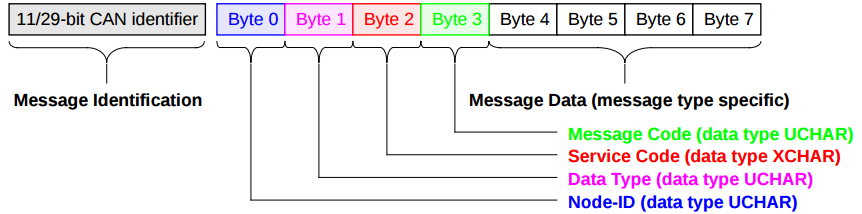
\includegraphics[scale=0.5]{images/Marco_teorico/CANAerospace_Message.png}
  \caption{Formato del mensaje de CANAerospace}
\label{fig:CANAerospaceMessage}
\end{figure}


